\documentclass[12pt, a4paper]{article}
% Some fancy symbols
\usepackage{textcomp}
\usepackage{stmaryrd}
\usepackage{cancel}

% Some fancy symbols
\usepackage{textcomp}
\usepackage{stmaryrd}


\usepackage{array}

% Math packages
\usepackage{amsmath,amsthm,amssymb, amsfonts, mathrsfs, dsfont, mathtools}
% \usepackage{mathtext}

\usepackage[bb=boondox]{mathalfa}
\usepackage{bm}

% To conrol figures:
\usepackage{subfig}
\usepackage{adjustbox}
\usepackage{placeins}
\usepackage{rotating}



\usepackage{lipsum}
\usepackage{psvectorian} % Insanely fancy text separators!


% Refs:
\usepackage{url}
\usepackage[backref]{hyperref}

% Fancier tables and lists
\usepackage{booktabs}
\usepackage{enumitem}
% Don't indent paragraphs, leave some space between them
\usepackage{parskip}
% Hide page number when page is empty
\usepackage{emptypage}


\usepackage{multicol}
\usepackage{xcolor}

\usepackage[normalem]{ulem}

% For beautiful code listings:
% \usepackage{minted}
\usepackage{listings}

\usepackage{csquotes} % For citations
\usepackage[framemethod=tikz]{mdframed} % For further information see: http://marcodaniel.github.io/mdframed/

% Plots
\usepackage{pgfplots} 
\pgfplotsset{width=10cm,compat=1.9} 

% Fonts
\usepackage{unicode-math}
% \setmathfont{TeX Gyre Termes Math}

\usepackage{fontspec}
\usepackage{polyglossia}

% Named references to sections in document:
\usepackage{nameref}


% \setmainfont{Times New Roman}
\setdefaultlanguage{russian}

\newfontfamily\cyrillicfont{Kurale}
\setmainfont[Ligatures=TeX]{Kurale}
\setmonofont{Fira Code}

% Common number sets
\newcommand{\sN}{{\mathbb{N}}}
\newcommand{\sZ}{{\mathbb{Z}}}
\newcommand{\sZp}{{\mathbb{Z}^{+}}}
\newcommand{\sQ}{{\mathbb{Q}}}
\newcommand{\sR}{{\mathbb{R}}}
\newcommand{\sRp}{{\mathbb{R^{+}}}}
\newcommand{\sC}{{\mathbb{C}}}
\newcommand{\sB}{{\mathbb{B}}}

% Math operators

\makeatletter
\newcommand\RedeclareMathOperator{%
  \@ifstar{\def\rmo@s{m}\rmo@redeclare}{\def\rmo@s{o}\rmo@redeclare}%
}
% this is taken from \renew@command
\newcommand\rmo@redeclare[2]{%
  \begingroup \escapechar\m@ne\xdef\@gtempa{{\string#1}}\endgroup
  \expandafter\@ifundefined\@gtempa
     {\@latex@error{\noexpand#1undefined}\@ehc}%
     \relax
  \expandafter\rmo@declmathop\rmo@s{#1}{#2}}
% This is just \@declmathop without \@ifdefinable
\newcommand\rmo@declmathop[3]{%
  \DeclareRobustCommand{#2}{\qopname\newmcodes@#1{#3}}%
}
\@onlypreamble\RedeclareMathOperator
\makeatother


% Correction:
\definecolor{correct_color}{HTML}{009900}
\newcommand\correction[2]{\ensuremath{\:}{\color{red}{#1}}\ensuremath{\to }{\color{correct_color}{#2}}\ensuremath{\:}}
\newcommand\inGreen[1]{{\color{correct_color}{#1}}}

% Roman numbers && fancy symbs:
\newcommand{\RNumb}[1]{{\uppercase\expandafter{\romannumeral #1\relax}}}
\newcommand\textbb[1]{{$\mathbb{#1}$}}



% MD framed environments:
\mdfsetup{skipabove=1em,skipbelow=0em}

% \mdfdefinestyle{definition}{%
%     linewidth=2pt,%
%     frametitlebackgroundcolor=white,
%     % innertopmargin=\topskip,
% }

\theoremstyle{definition}
\newmdtheoremenv[nobreak=true]{definition}{Определение}
\newmdtheoremenv[nobreak=true]{theorem}{Теорема}
\newmdtheoremenv[nobreak=true]{lemma}{Лемма}
\newmdtheoremenv[nobreak=true]{problem}{Задача}
\newmdtheoremenv[nobreak=true]{property}{Свойство}
\newmdtheoremenv[nobreak=true]{statement}{Утверждение}
\newmdtheoremenv[nobreak=true]{corollary}{Следствие}
\newtheorem*{note}{Замечание}
\newtheorem*{example}{Пример}

% To mark logical parts
\newcommand{\existence}{{\circled{$\exists$}}}
\newcommand{\uniqueness}{{\circled{$\hspace{0.5px}!$}}}
\newcommand{\rightimp}{{\circled{$\Rightarrow$}}}
\newcommand{\leftimp}{{\circled{$\Leftarrow$}}}


% Useful symbols:
\renewcommand{\qed}{\ensuremath{\blacksquare}}
\renewcommand{\vec}[1]{\overrightarrow{#1}}
\newcommand{\eqdef}{\overset{\mathrm{def}}{=\joinrel=}}
\newcommand{\isdef}{\overset{\mathrm{def}}{\Longleftrightarrow}}
\newcommand{\inductdots}{\ensuremath{\overset{induction}{\cdots}}}

% Matrix's determinant
\newenvironment{detmatrix}
{
  \left|\begin{matrix}
}{
  \end{matrix}\right|
}

\newenvironment{complex}
{
  \left[\begin{gathered}
}{
  \end{gathered}\right.
}


\newcommand{\nl}{$~$\\}

\newcommand{\tit}{\maketitle\newpage}
\newcommand{\tittoc}{\tit\tableofcontents\newpage}


\newcommand{\vova}{  
    Латыпов Владимир (конспектор)\\
    {\small \texttt{t.me/donRumata03}, \texttt{github.com/donRumata03}, \texttt{donrumata03@gmail.com}}
}


\usepackage{tikz}
\newcommand{\circled}[1]{\tikz[baseline=(char.base)]{
            \node[shape=circle,draw,inner sep=2pt] (char) {#1};}}

\newcommand{\contradiction}{\circled{!!!}}

% Make especially big math:

\makeatletter
\newcommand{\biggg}{\bBigg@\thr@@}
\newcommand{\Biggg}{\bBigg@{4.5}}
\def\bigggl{\mathopen\biggg}
\def\bigggm{\mathrel\biggg}
\def\bigggr{\mathclose\biggg}
\def\Bigggl{\mathopen\Biggg}
\def\Bigggm{\mathrel\Biggg}
\def\Bigggr{\mathclose\Biggg}
\makeatother


% Texts dividers:

\newcommand{\ornamentleft}{%
    \psvectorian[width=2em]{2}%
}
\newcommand{\ornamentright}{%
    \psvectorian[width=2em,mirror]{2}%
}
\newcommand{\ornamentbreak}{%
    \begin{center}
    \ornamentleft\quad\ornamentright
    \end{center}%
}
\newcommand{\ornamentheader}[1]{%
    \begin{center}
    \ornamentleft
    \quad{\large\emph{#1}}\quad % style as desired
    \ornamentright
    \end{center}%
}


% Math operators

\DeclareMathOperator{\sgn}{sgn}
\DeclareMathOperator{\id}{id}
\DeclareMathOperator{\rg}{rg}
\DeclareMathOperator{\determinant}{det}

\DeclareMathOperator{\Aut}{Aut}

\DeclareMathOperator{\Sim}{Sim}
\DeclareMathOperator{\Alt}{Alt}



\DeclareMathOperator{\Int}{Int}
\DeclareMathOperator{\Cl}{Cl}
\DeclareMathOperator{\Ext}{Ext}
\DeclareMathOperator{\Fr}{Fr}


\RedeclareMathOperator{\Re}{Re}
\RedeclareMathOperator{\Im}{Im}


\DeclareMathOperator{\Img}{Im}
\DeclareMathOperator{\Ker}{Ker}
\DeclareMathOperator{\Lin}{Lin}
\DeclareMathOperator{\Span}{span}

\DeclareMathOperator{\tr}{tr}
\DeclareMathOperator{\conj}{conj}
\DeclareMathOperator{\diag}{diag}

\expandafter\let\expandafter\originald\csname\encodingdefault\string\d\endcsname
\DeclareRobustCommand*\d
  {\ifmmode\mathop{}\!\mathrm{d}\else\expandafter\originald\fi}

\newcommand\restr[2]{{% we make the whole thing an ordinary symbol
  \left.\kern-\nulldelimiterspace % automatically resize the bar with \right
  #1 % the function
  \vphantom{\big|} % pretend it's a little taller at normal size
  \right|_{#2} % this is the delimiter
  }}

\newcommand{\splitdoc}{\noindent\makebox[\linewidth]{\rule{\paperwidth}{0.4pt}}}

% \newcommand{\hm}[1]{#1\nobreak\discretionary{}{\hbox{\ensuremath{#1}}}{}}


\usepackage{geometry}
\geometry{
    a4paper,
    left=13mm,
    right=13mm,
    top=15mm,
    bottom=10mm
}

\graphicspath{{res/}}


\title{Теорвер. Домашнее задание №2 \\ \large Условная вероятность} 

\author{
  Латыпов Владимир
}

\date{\today}



\begin{document}
\maketitle
\newpage

\section{Независимость в подпространстве}

\begin{enumerate}
    \item Выберем такое $p_A$, что $\forall B, C \subset A: p_A(B | C) = p_\Omega(B | C)$.
    
    \begin{gather}
        p_A(B | C) \eqdef \frac{p_A(BC)}{p_A(C)} \\
        p_\Omega(B | C) \eqdef \frac{p(BC)}{p(C)}
    \end{gather}

    Если мы возьмём $p_A(D) = p(D | A) = \frac{p(DA)}{p(A)} = \frac{p(D)}{p(A)}, D \subset A$, 
    то аксиомы будут, тривиально, выполнены,
    а числитель и знаменатель дроби $\frac{p_A(BC)}{p_A(C)}$ отнормируется в $p(A)$ раз, 
    значит, требуемое соотношение тоже выполнено.

    \item Пусть $p(A) = 1$. Докажем, что $\forall B \in \Omega p(B | A) = p(B)$.
    
    \begin{multline}
        p(B | A) \eqdef \frac{p(AB)}{p(A)} = p(AB) = \\
        p((\Omega \backslash (\Omega \backslash A))B) = \\
        p(\Omega B + \backslash (\Omega \backslash A) B) \underset{disj} = \\
        p(B) - p((\Omega \backslash A) B) = p(B)
    \end{multline}

    \item \begin{enumerate}
        \item Верно ли, что независимость в подпространстве 
        влечёт независимость во всём пространстве?
        
        Если $B, C \subset A$ независимы, $p(BC) = p(B) p(C)$. 

        \begin{gather}
            p_A(BC) = \frac{p(BC)}{p(A)} \\
            p_A(B)p_A(C) = \frac{p(B)p(C)}{p^2(A)} = \frac{p(BC)}{p^2(A)}
        \end{gather}
        
        Что верно только если $p(A) = 1$ или кто-то из $B, C$ — пустой: только в паталогическом случае.

        Берём контрпример от балды: $B, C$: в Питере, Москве идёт дождь. $A = B \cup C$.

        \item Верна ли обратная импликация? Ровно те же формулы.
        
        \item Выполняется ли такая хрень для попарно независимых событий.
        
        $p_A(AB \cdot AC) = p_A(ABC) = \frac{p(ABC)}{p(A)} \eqOrNot p_A(AB)p_A(AC) = \frac{p(AB)p(AC)}{p^2(A)} = p(B)p(C)$.

        То есть требование задачи — чтобы не были зависимы в совокупности, а условие — лишь попарная зависимость.

        Контрпример:

        \begin{sidewaysfigure}[h!]
            \centering
            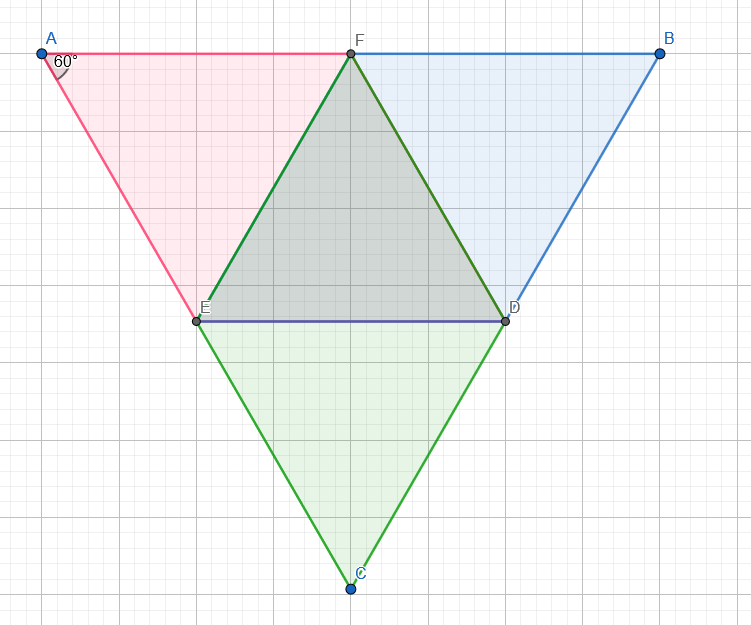
\includegraphics[width=\paperwidth]{res/counterexample.png}
            \caption{Контрпример}
            \label{fig:counterexample}
        \end{sidewaysfigure}
        \FloatBarrier
    \end{enumerate}
\end{enumerate}


\section{\textit{Простая} задача}

$p(k) = a^{k - 1} \underbrace{\frac{1 - a}{1 - a^6}}_c$

Чётные: $E = \{2, 4, 6\}$.

Не простые: $N = \{1, 4, 6\}$.

\begin{equation}
    P(EN) = P(\{4, 6\}) = p(N) - p_1 = p(E) - p_2 = c(a^3 + a^5)
\end{equation}

\begin{equation}
    p(E)p(N) = c(a^1 + a^3 + a^5) \cdot c(a^0 + a^3 + a^5) = (c a + P(EN))(c + P(EN))
\end{equation}

$E, N$ независимы $\Leftrightarrow$

\begin{equation}
    P(EN) = r = (ca + r)(c + r) = c^2 a + r(c + ca) + r^2
\end{equation}

То есть должно быть: $r^2 + r (ca + c - 1) + c^2 a = 0$.


\begin{enumerate}
    \item $a = \sqrt{\frac{-2+\sqrt{7}}{2}}$.
    
    \begin{gather}
        c = \frac{1 - \sqrt{\frac12 (\sqrt{7} - 2)}}{1 - \frac18 (\sqrt{7} - 2)^3} \\
        r = c(a^3 + a^5) = \frac{\left(1-\sqrt{\frac{1}{2}(\sqrt{7}-2)}\right)\left(\frac{(\sqrt{7}-2)^{3 / 2}}{2 \sqrt{2}}+\frac{(\sqrt{7}-2)^{5 / 2}}{4 \sqrt{2}}\right)}{1-\frac{1}{8}(\sqrt{7}-2)^3}
    \end{gather}

    Получим гадость (не ноль): \url{https://www.wolframalpha.com/input?i=find+r%5E2+%2B+r+%28ca+%2B+c+-+1%29+%2B+c%5E2+a+for+a%3Dsqrt%281%2F2+%28sqrt%287%29+-+2%29%29%2C+c%3D%281+-+a%29%2F%281+-+a%5E6%29%2C+r+%3D+c*+%28a%5E3+%2B+a%5E5%29}.


    \item Получим ноль: \url{https://www.wolframalpha.com/input?i=find+r%5E2+%2B+r+%28ca+%2B+c+-+1%29+%2B+c%5E2+a+for+a%3Dsqrt%281%2F2+%28sqrt%285%29+-+1%29%29%2C+c%3D%281+-+a%29%2F%281+-+a%5E6%29%2C+r+%3D+c*+%28a%5E3+%2B+a%5E5%29}.
\end{enumerate}


\section{Контрпримеры}

\begin{itemize}
    \item Да, $A = \varnothing$.
    \item $B: 2 × 2 = 4$, $A$ — злая воля сумасшедшего диктатора.
    \item $A = B:$ Я сегодня пойду гулять.
\end{itemize}


\section{Неравенства}

\begin{enumerate}
    \item Буль: \begin{itemize}
        \item Буль1 [aka Полуаддитивность меры]: $P\left(\bigcup_{i=1}^n A_i\right) \leqslant \sum_{i=1}^n P\left(A_i\right)$. 
        
        Заведём $B_i = A_i \backslash \bigcup_{j=1}^{i - 1} A_j$. Тогда они дизъюнктны, $B_i \subset A_i$ и имеют то же объединение.

        \begin{equation}
            P\left(\bigcup_{i=1}^n A_i\right) = P\left(\bigsqcup_{i=1}^n B_i\right) = \sum_{i=1}^n P\left(B_i\right) \leqslant \sum_{i=1}^n P\left(A_i\right)
        \end{equation}
        
        \item Буль2: $P\left(\bigcap_{i=1}^n A_i\right) \geqslant 1-\sum_{i=1}^n P\left(\bar{A}_i\right)$.
        
        \begin{equation}
            P\left(\bigcap_{i=1}^n A_i\right) = P\left(\overline{\bigcup_{i=1}^n \overline{A_i}}\right) = 1 - P\left(\bigcup_{i=1}^n \overline{A_i}\right) \geqslant 1 - \sum_{i=1}^n P\left(\overline{A_i}\right)
        \end{equation}

    \end{itemize}

    \item Буль-Буль
    
    \begin{equation}
        P\left(\bigcap_{i=1}^n A_i\right) \geqslant 1 - \sum_{i=1}^n P\left(\overline{A_i}\right) = 
        1 - \left(n - \sum_{i=1}^n P\left(A_i\right)\right) = \sum_{i=1}^n P\left(A_i\right) - (n - 1)
    \end{equation}

    \item Буль-Буль-Буль [Куниасс]
    
    \begin{equation}
        (!) \forall k P\left(\bigcup_{i=1}^n A_i\right) \leqslant \sum_{i=1}^n P\left(A_i\right) - \sum_{i \neq k} P\left(A_i \cap A_k\right)
    \end{equation}

    НУО, $k = 1$. 


    \begin{multline}
        P\left(\bigcup_{i=1}^n A_i\right) = P\left(\left(A_1 \backslash \bigcup_{i=2}^n A_i \right) \cup \bigcup_{i=2}^n A_i\right) \leqslant \\
        P(A_1) - \sum_{i \neq k} P\left(A_i \cap A_k\right) + \sum_{i=2}^n P\left(A_i\right) = \\
        \sum_{i=1}^n P\left(A_i\right) - \sum_{i \neq k} P\left(A_i \cap A_k\right)
    \end{multline}
\end{enumerate}

\section{Априорные шары}

Заметим, что по определению условной вероятности, $P(B_j | A_k) = \frac{p(B_j \cap A_k)}{p(A_k)}$,
а это ровно числа, фигурирующие в подсказке. Если поделить одно на другое, получится роавно то, что надо.

Равенства из подсказки получаются, если сначала \textit{выбрать} позиции белых шаров,
а потом расставить (с возвратом или без) конкретные белые/цветные шары на них.
В первом случае вылезает обычная степень, втором — убывающая.


\section{„Добавленный“ белый шар}

$A$ — оставшийся шар — белый.
$B$ — вытащили белый.

$W$ — добавили белый шар.

\begin{equation}
    P(A | B) = \frac{p(AB)}{p(B)} = \frac{\frac{1}{2}}{p(W)p(B | W) + p(\overline{W})p(B | \overline{W})} =
    \frac{\frac{1}{2}}{½ \cdot 1 + ½\cdot ½} = \frac{\frac{1}{2}}{\frac 34} = \frac 46 = \frac 23
\end{equation}

\section{А было ли письмо?}

$A$ — письмо есть. $B$ — письмо есть в первых 7-и.



\begin{equation}
    p(A | \overline{B}) = p(A) \frac{p(\overline{B} | A)}{p(\overline{B})} = p \frac{\frac{1}{8}}{1 - \frac{7}{8}p} = \frac{p}{8 - 7p}
\end{equation}


Заметим, что без дополниельной информации, вероятность найти письмо в последнем ящике была бы $\frac{p}{8}$, а так она повышается,
причём при больших $p$ повышается сильнее.


\section{Совисимая незакупность}

Разобъём на $2^n$ дизъюнктных событий $\bigcap A_i^{[\complement]}$,
каждое из которых непусто, тем самым покажем,
что как минимум $2^n$ различных элементов пространства точно есть.

\begin{lemma}
    Если события $\{B_i\}^n_{i = 0}$ независимы в совокупности,
    то события $B_1, … \overline{B_k}, … B_n$ — тоже независимы в совокупности.
\end{lemma}

\begin{proof}
    Если $k \notin I \subset [1; n]$, $p\left(\bigcap_{i \in I} B_i'\right) = p\left(\bigcap_{i \in I} B_i\right) = \prod_{i \in I} p(B_i)$ (ничего не меняется).

    Если $k \in I \subset [1; n]$,
    \begin{multline}
        p\left(\bigcap_{i \in I} B'_i\right)
        = p\left(\overline{B_i} \cap \bigcap_{i \in (I \backslash \{k\})} B_i\right)
        = p\left(\bigcap_{i \in (I \backslash \{k\})} B_i\right) - p\left(\bigcap_{i \in I} B_i\right) \\
        = \prod_{i \in (I \backslash \{k\})} B_i - \prod_{i \in I} B_i \\
        = (1 - p(B_i)) \prod_{i \in (I \backslash \{k\})} B_i
        = \prod_{i \in I} p(B'_i)
    \end{multline}
\end{proof}

А значит, для любой битовой маски окажется, что событие $\bigcap A_i^{[\complement]}$, где дополнения стоят на местах нулей,
имеет ненулевую вероятность (каждый из сомножителетей не ноль по условию):

\begin{equation}
    \prod^n_{i = 0} \begin{cases}
        p(A_i) & i \in I \\
        1 - p(A_i) & i \notin I
    \end{cases}
\end{equation}

Итак, получили $2^n$ дизъюнктных непустых событий $\bigcap A_i^{[\complement]}$

\begin{remark}
    Почему эти пересечения событий дизъюнктно разбивают $\Omega$?

    \begin{proof}
    Возьмём точку $x \in \Omega$ и докажем, что что существует единственная битовая маска, содержащая её.
    
    \existence Выберем такое $I(x)$, что $i \in I$ при $x \in A_i$. Тогда $x \in \bigcap^n_{i = 0} \begin{cases}
        p(A_i) & i \in I \\
        1 - p(A_i) & i \notin I
    \end{cases}$.

    \uniqueness Никакому другому пересечению такого вида $x$ не принадлежит, так как у другого найдётся место,
    в котором требование противоположно таковому в $I(x)$ тогда $x$ ему не удовлетворяет.
\end{proof}

\end{remark}

Пример для $2^n$ — гиперкуб с событиями $A_i$: $i$-й бит = $1$.

\end{document}
